\documentclass[border=4pt,tikz]{standalone}
\usepackage{tikz}
\usetikzlibrary{arrows.meta,positioning,shapes.geometric}
\begin{document}
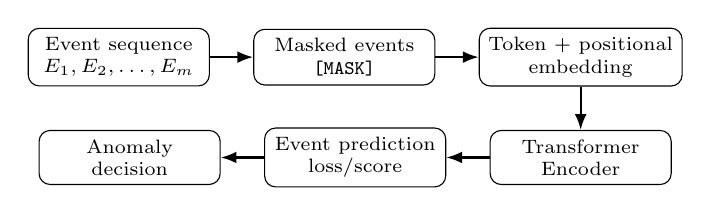
\begin{tikzpicture}[
    node distance=0.55cm,
    box/.style={rectangle, draw, rounded corners, align=center, minimum width=2.3cm, minimum height=0.62cm, font=\scriptsize},
    arrow/.style={-{Latex[length=2mm]}, thick}
]
\node[box] (seq) {Event sequence\\$E_1,E_2,\ldots,E_m$};
\node[box, right=of seq] (mask) {Masked events\\\texttt{[MASK]}};
\node[box, right=of mask] (emb) {Token + positional\\embedding};
\node[box, below=of emb] (enc) {Transformer\\Encoder};
\node[box, left=of enc] (pred) {Event prediction\\loss/score};
\node[box, left=of pred] (alert) {Anomaly\\decision};
\draw[arrow] (seq) -- (mask);
\draw[arrow] (mask) -- (emb);
\draw[arrow] (emb) -- (enc);
\draw[arrow] (enc) -- (pred);
\draw[arrow] (pred) -- (alert);
\end{tikzpicture}
\end{document}
